The intention of this report is to investigate preliminary data coming from the ITS and MFT in Run 3. The order of the discussion in this section will follow the order that we tackled things. This is done to show both the progression of our knowledge as well as to try to clarify some of the explanations in previous sections as the only way to truly understand some things is through example. 

\subsection{The Data}
The data analysed in this report was taken in October 2021, where protons were collided at a centre of mass energy of \SI{900}{\giga\electronvolt}. This is not an energy that we expect to use for physics research but it allows us to look at how the detectors are performing with more lightweight data, simply because there will be fewer particles created in the collisions and thus less data to work with. We are using runs 505548 and 505645. In this case, a run specifies a period of data taking for which all global settings remain the same. All further plots, unless specified otherwise, will include both runs.


\subsection{Initial MFT Analysis}
In the AOD data model there is a table called \texttt{MFTTracks} which contains the tracks detected in the MFT. When we began this analysis, only two reconstruction passes had been run on the data and while the MFT was switched on for the runs, the \texttt{MFTTracks} table had not been populated. We thus had to wait for pass 3 and we spent that time getting familiar with the analysis framework as described in \cref{sec:AnalysingWithO2}. With pass 3 available, the plots in \cref{fig:MFT_1D_pass3} were able to be created. The variables plotted are all available as static or dynamic columns in the AOD structure so no complicated analysis was needed to obtain them. 

\begin{figure}[h]%
    \centering
    \begin{subfigure}[t]{.49\linewidth}
        \centering
        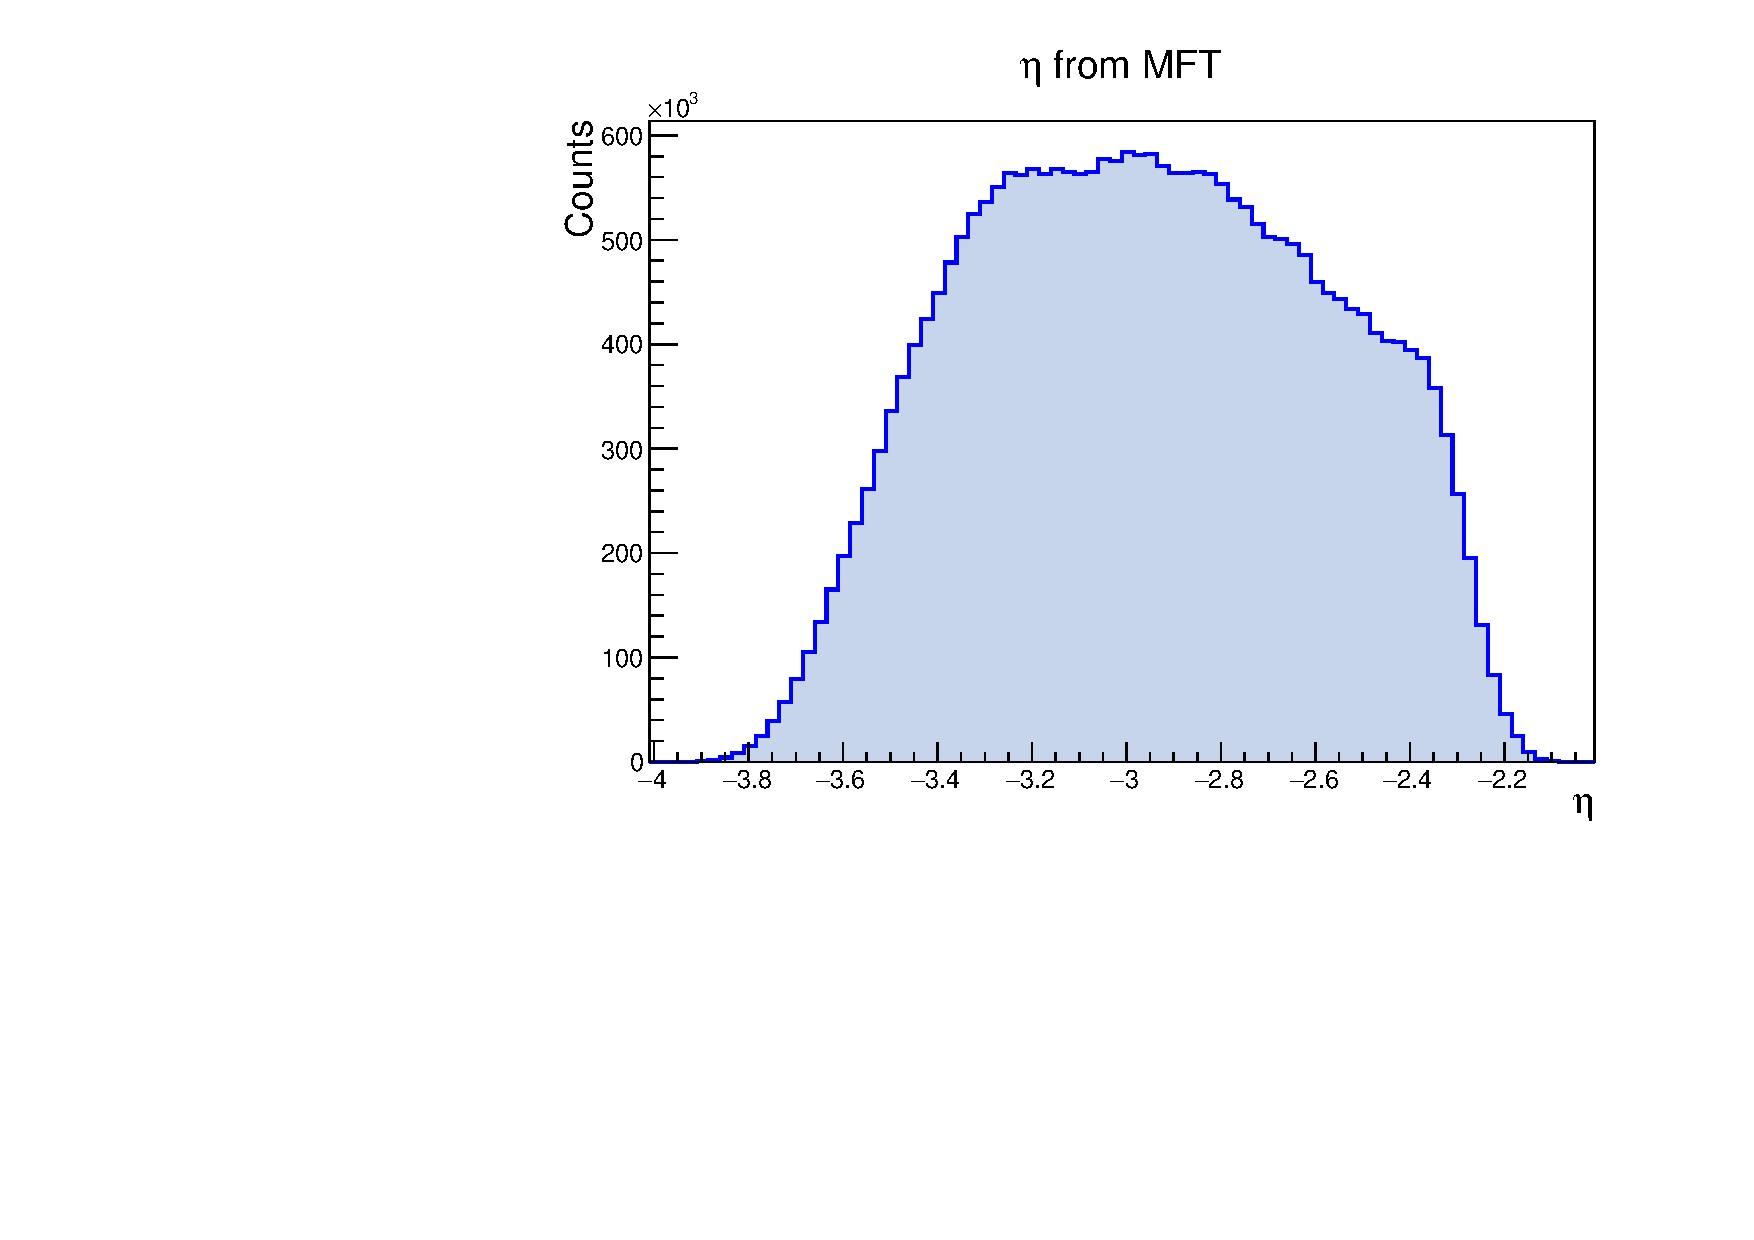
\includegraphics[width=\linewidth]{Plots/pass3_MFT/MFTeta_pass3.pdf}
        \caption{$\eta$ of tracks detected in the MFT. }
        \label{fig:MFTeta_pass3}
    \end{subfigure}
    \hfill
    \begin{subfigure}[t]{.49\linewidth}
        \centering
        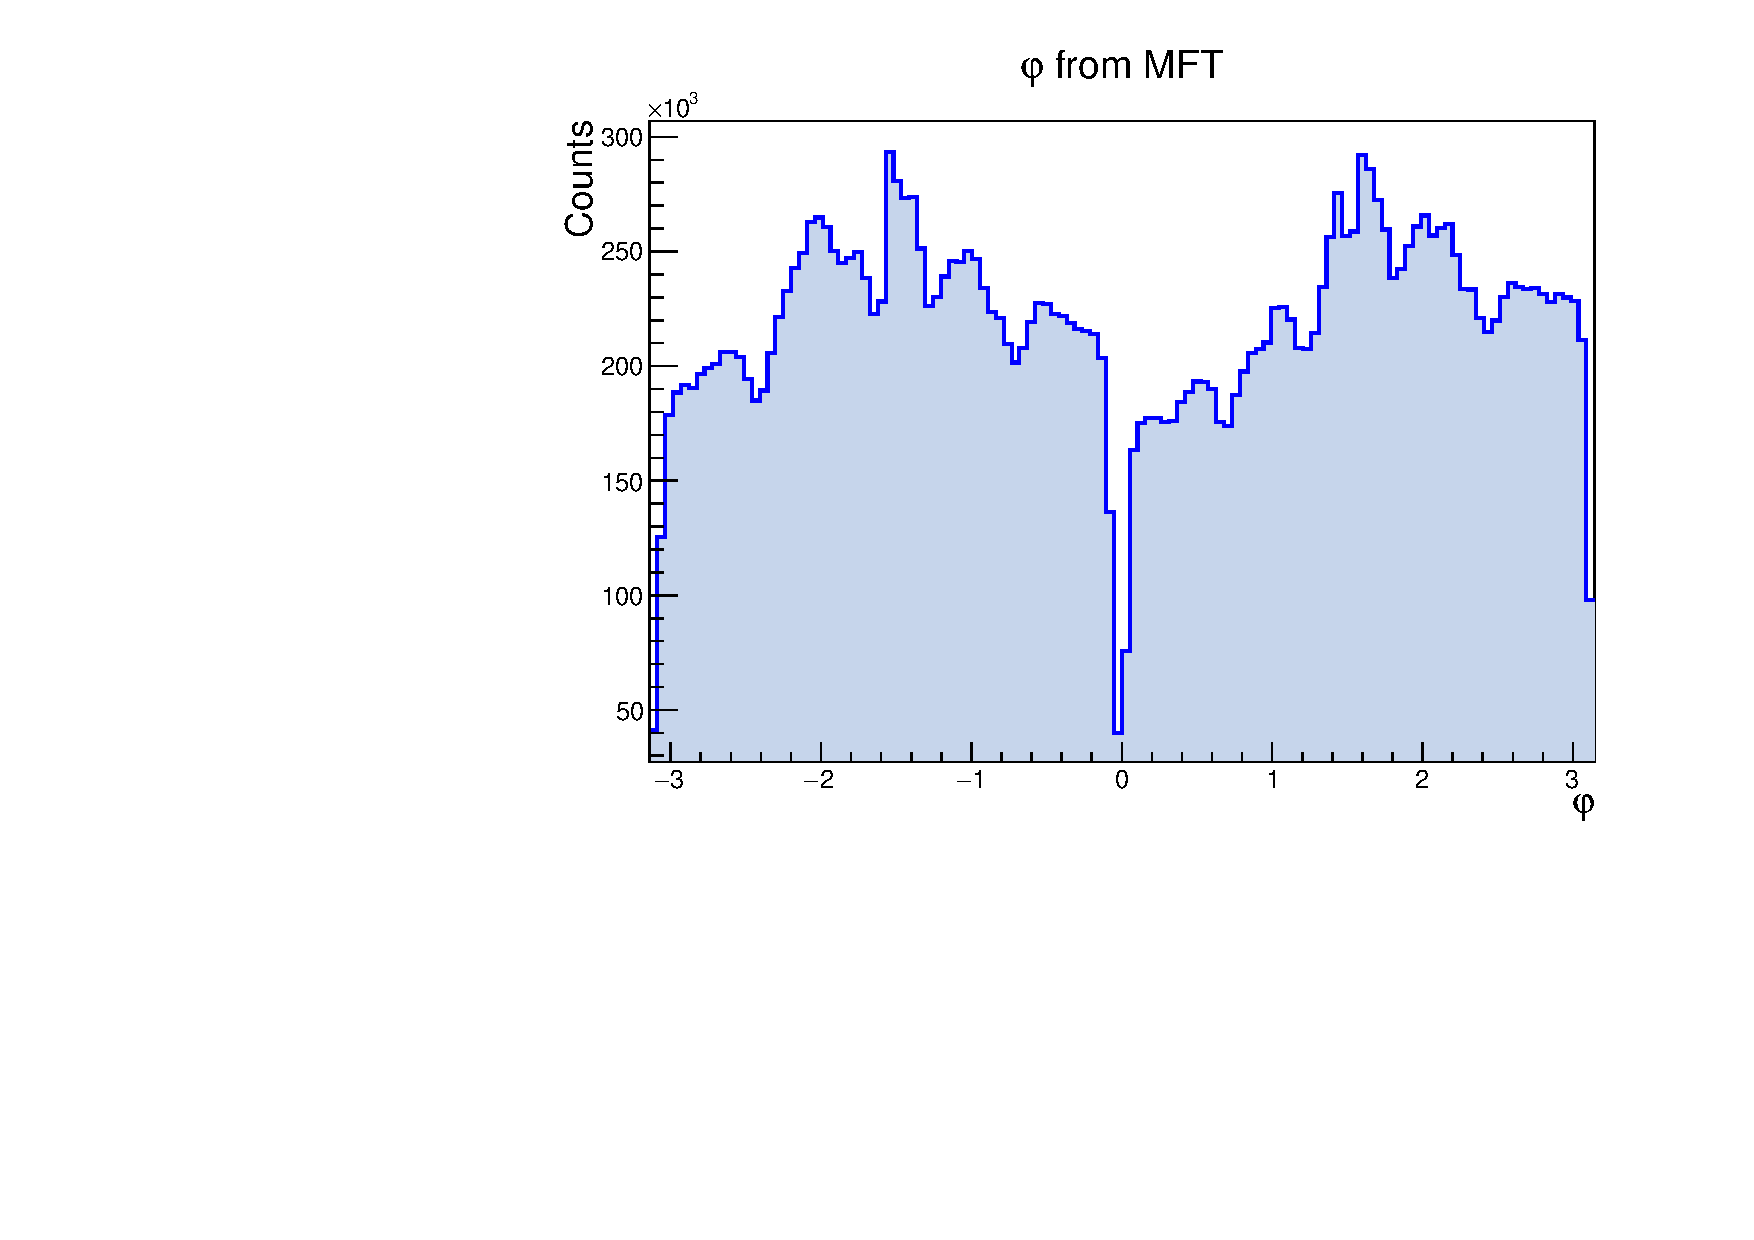
\includegraphics[width=\linewidth]{Plots/pass3_MFT/phi_pass3.pdf}
        \caption{$\varphi$ of tracks detected in the MFT. Note the range of $\varphi$.}
        \label{fig:MFTphi_pass3}
    \end{subfigure}
    \begin{subfigure}[t]{.49\linewidth}
        \centering
        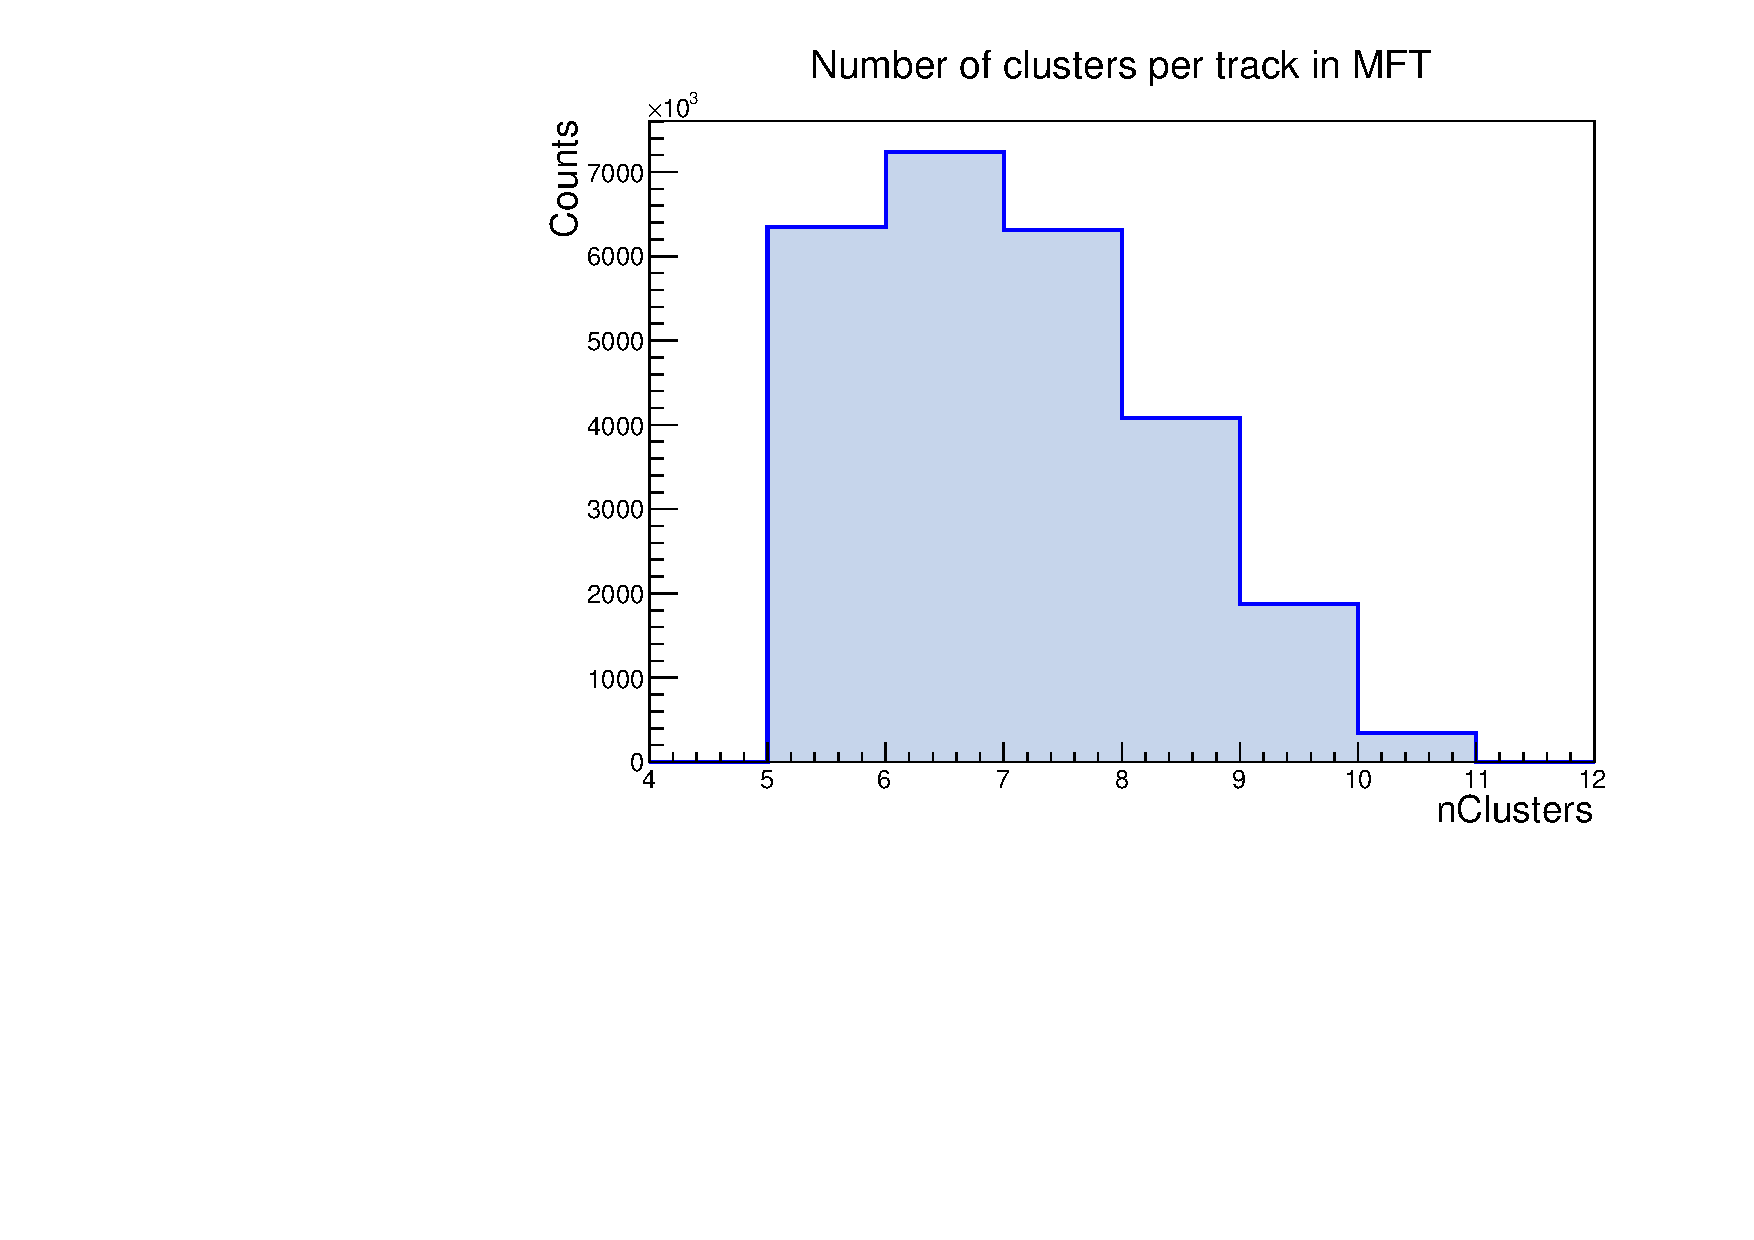
\includegraphics[width=\linewidth]{Plots/pass3_MFT/nClusters_pass3.pdf}
        \caption{Number of clusters per track detected in the MFT. Note the cut-off at 5.}
        \label{fig:MFTnClusters_pass3}
    \end{subfigure}
    \hfill
    \begin{subfigure}[t]{.49\linewidth}
        \centering
        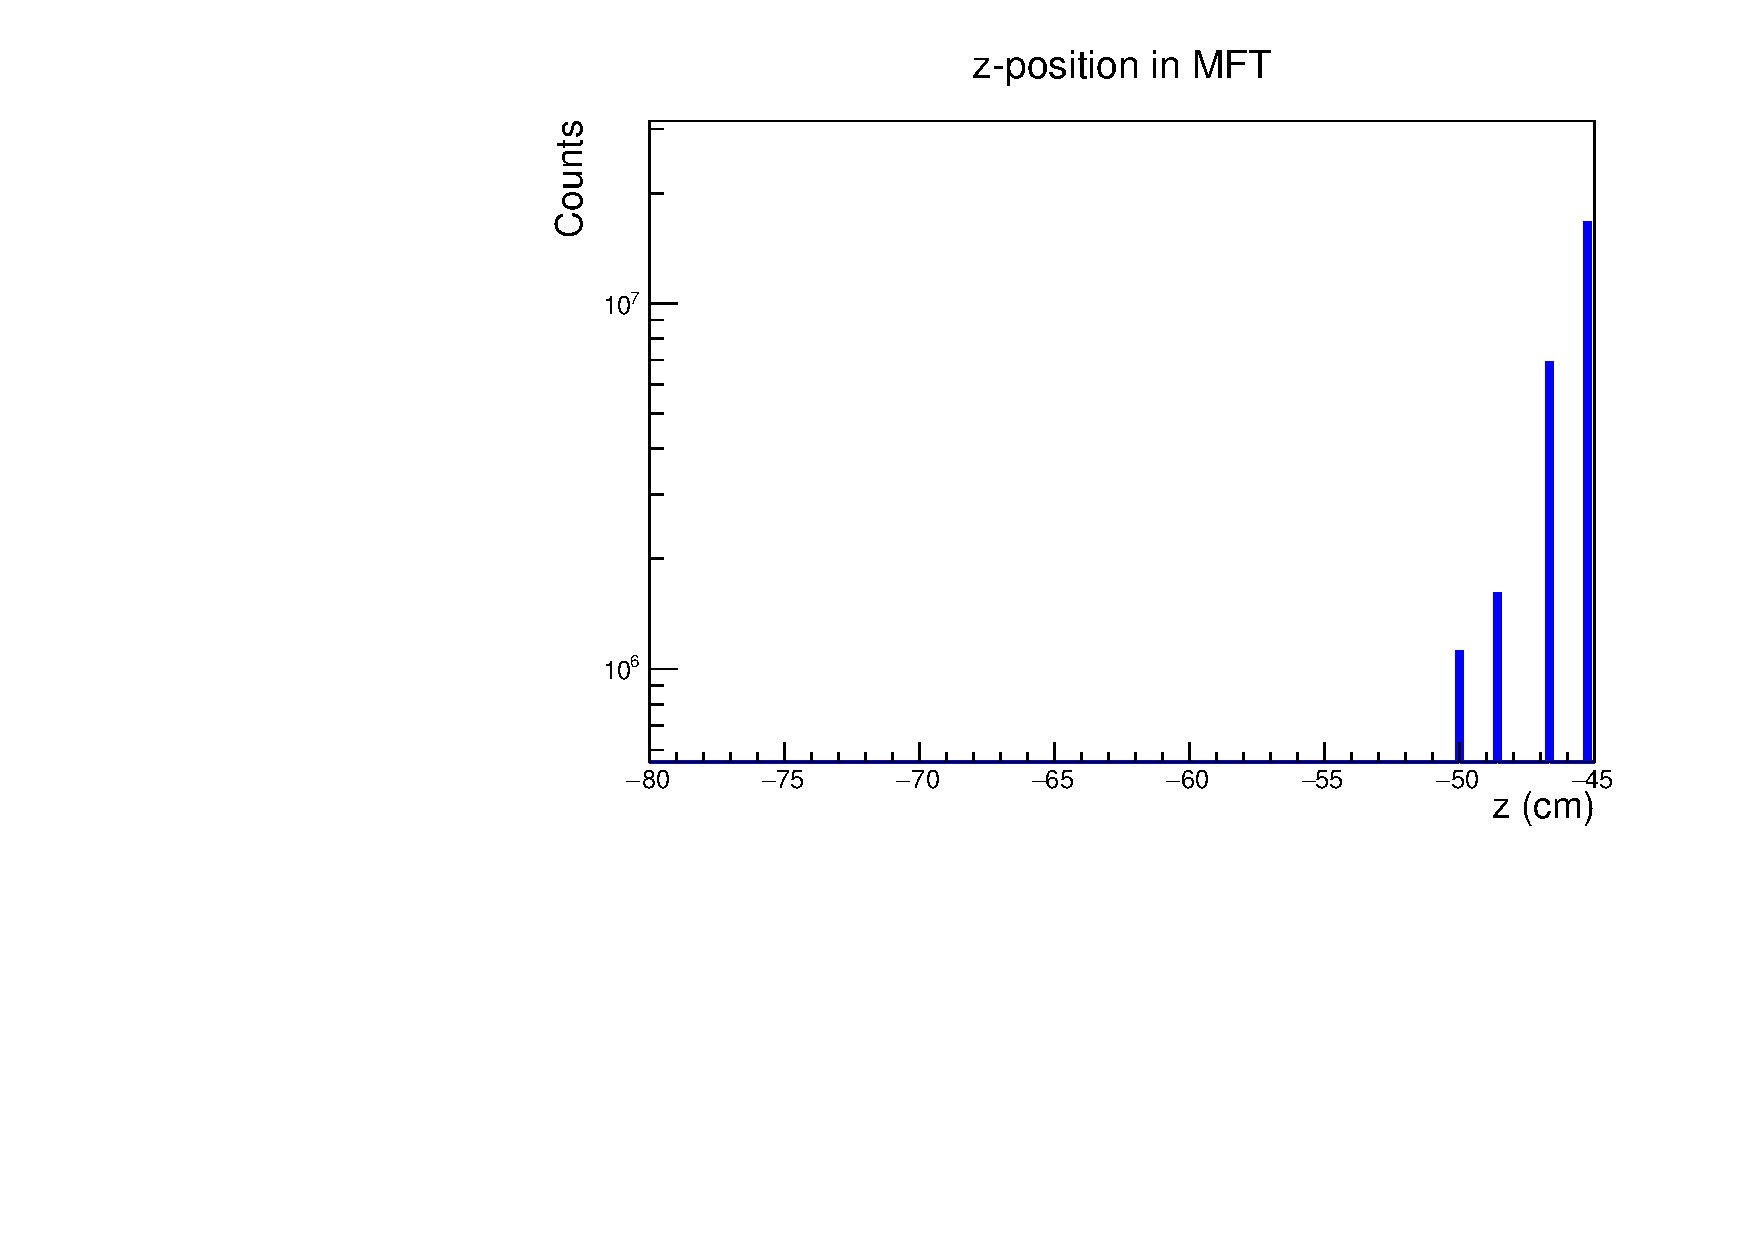
\includegraphics[width=\linewidth]{Plots/pass3_MFT/Z_MFT_pass3.pdf}
        \caption{$z$-position of first hit in the MFT. Note how the $z$ range covers the whole MFT but only the first 4 detector planes have hits.}
        \label{fig:Z_MFT_pass3}
    \end{subfigure}
\caption{1D histograms for some kinematic variables as well as the number of clusters per track in the MFT. Data from reconstruction pass 3. }
\label{fig:MFT_1D_pass3}
\end{figure}

Starting with $\eta$, we see the distribution is lopsided to the lower $\eta$ values but it's not as smooth in the middle as we might expect from a detector with continuous sensitive material in those regions. We will investigate this more in \cref{sec:comapring}. The $\varphi$ plot shows the structure of the MFT quite well. The valley at the centre shows the gap between the top and bottom half-disks and the spikes come from the fact that the sensitive area of each disk is not perfectly circular, so there will be directions that can detect more tracks than others. 

The number of clusters per track is interesting. As was mentioned in \cref{sec:MFT_Theory}, the MFT requires a track to be detected in 4 out of the 5 disks in order to be considered a track. The translation of that statement into number of clusters per track is a bit unclear but we might expect that the minimum number of clusters per track should be 4 as each disk has 2 planes but the track only needs to have a cluster in one of them to count towards the 4 out of 5. However, what we see in \cref{fig:MFTnClusters_pass3} is a minimum of 5 clusters per track. This might be down to a choice made in the reconstruction process to instead require that all 5 disks detect the track before it is accepted. It could also be due to a physical limitation where it's simply not possible for 4 disks to detect a track and not see clusters in 5 disks. At the point of writing, we have not been able to determine the reason for this as the details of reconstruction are near impossible to find.

Interpreting \cref{fig:Z_MFT_pass3} was its own adventure. The documentation for the AOD data model is unclear what gets calculated for the $z$ column in the \texttt{MFTTracks} table, but after much consideration we believe that it represents the $z$-position of the first hit (or cluster) of a given track in the MFT. We see that after the fourth plane, i.e. the second disk, there is no data. This supports the fact that 4 out of 5 disks are required to accept a track as having a first hit in the third disk will obviously never result in a track hitting 4 disks. This information seems to be contradicting the information from \cref{fig:MFTnClusters_pass3} but we regrettably have no resolution to the situation.

\begin{figure}[h]
    \begin{center}
        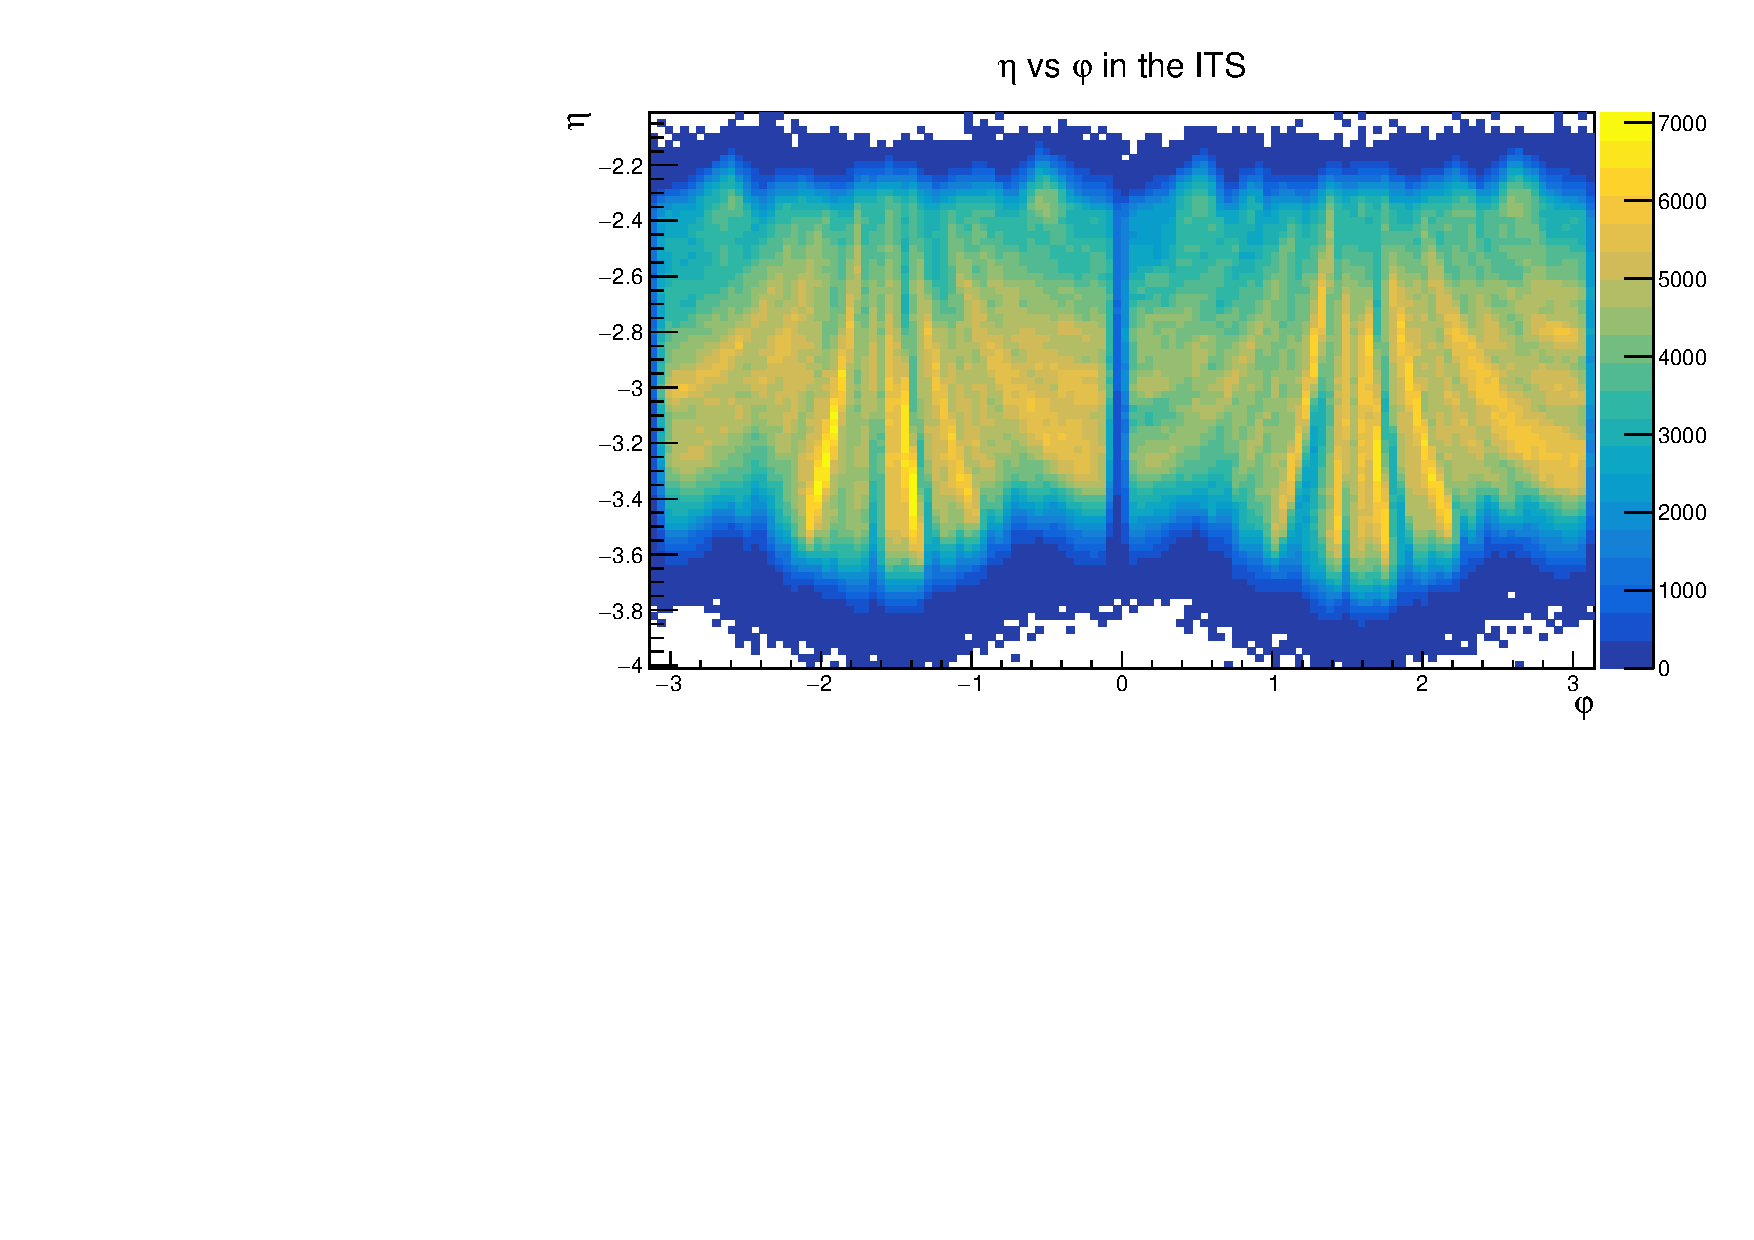
\includegraphics[width=.8\textwidth]{Plots/pass3_MFT/eta_phi_pass3.pdf}
        \caption{caption}
        \label{fig:eta_phi_pass3}
    \end{center}
\end{figure}


\begin{figure}[h]%
    \centering
    \begin{subfigure}[t]{.45\linewidth}
        \centering
        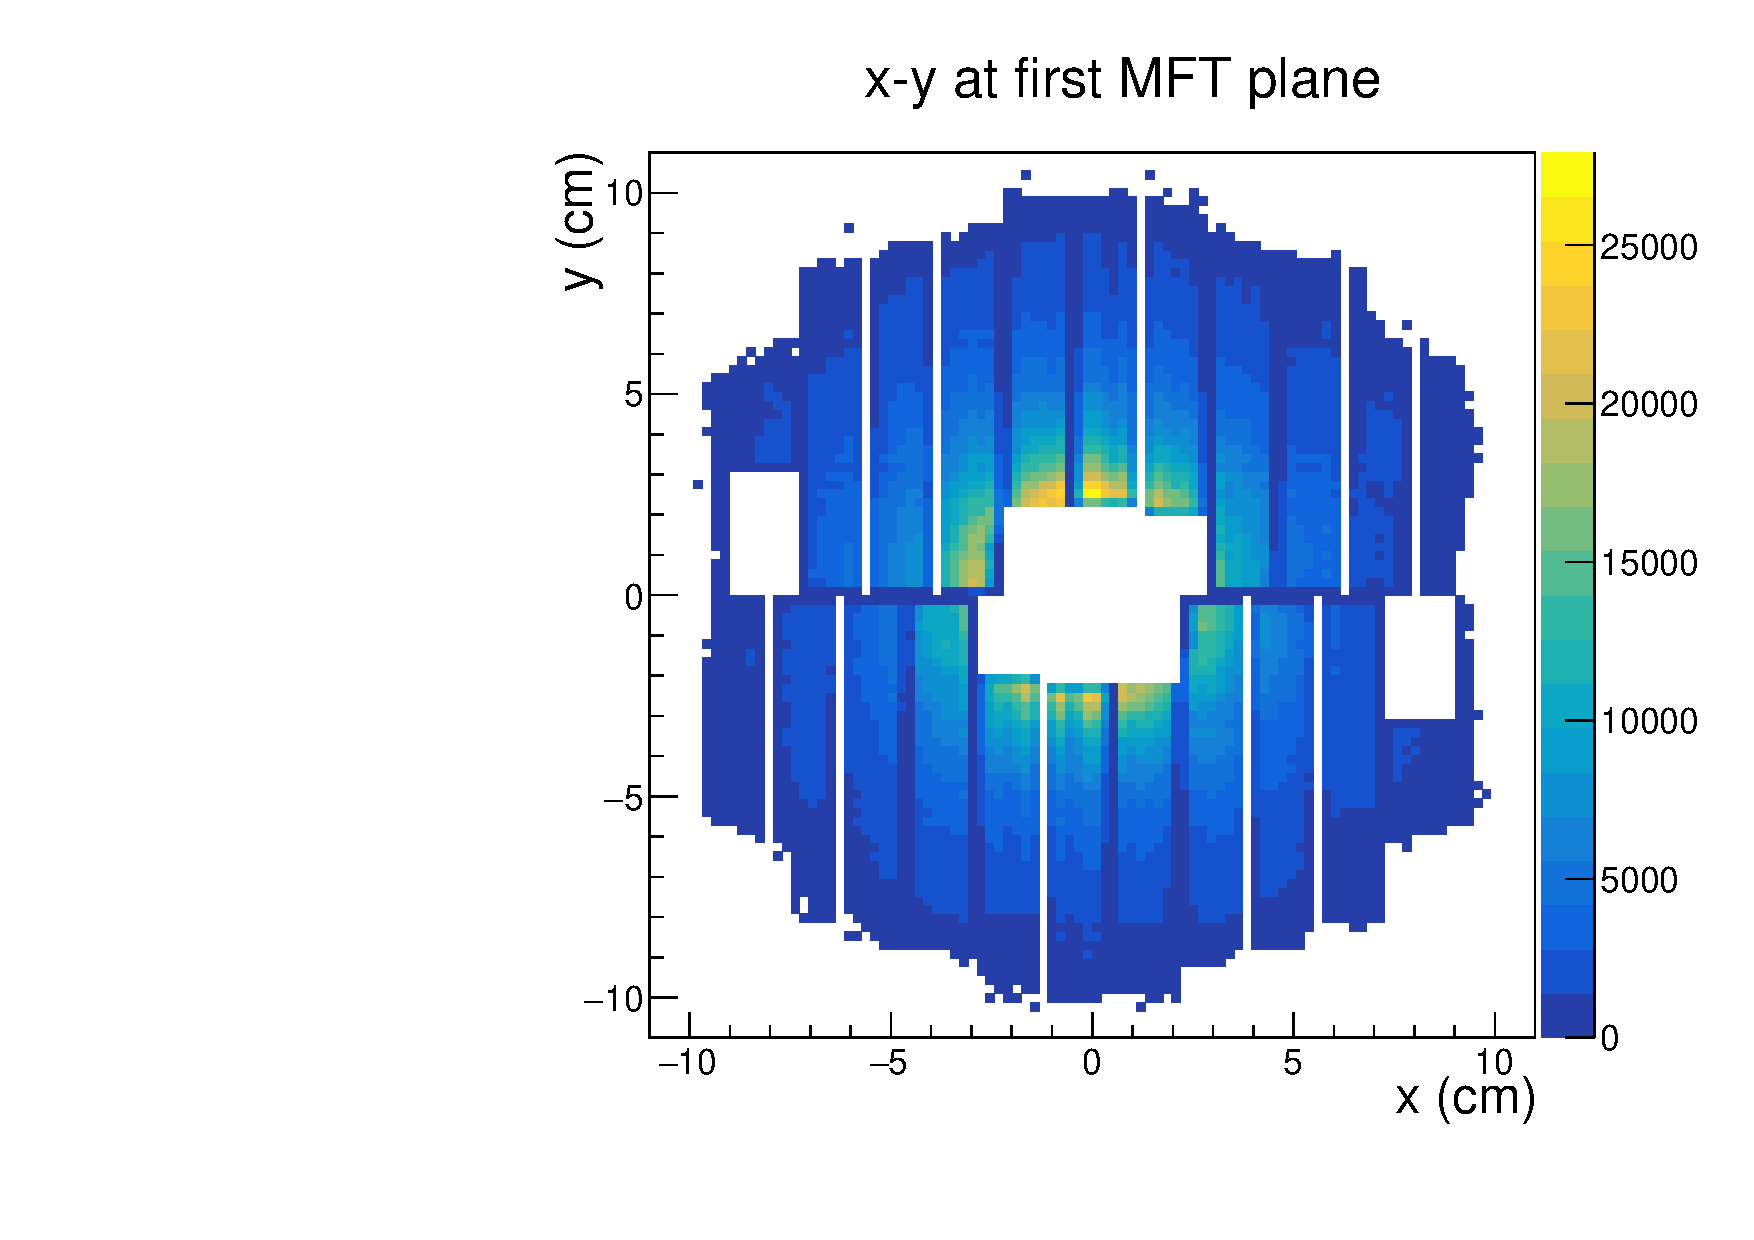
\includegraphics[width=\linewidth]{Plots/pass3_MFT/x_y_1_pass3.pdf}
        \caption{}
        \label{}
    \end{subfigure}
    \hfill
    \begin{subfigure}[t]{.45\linewidth}
        \centering
        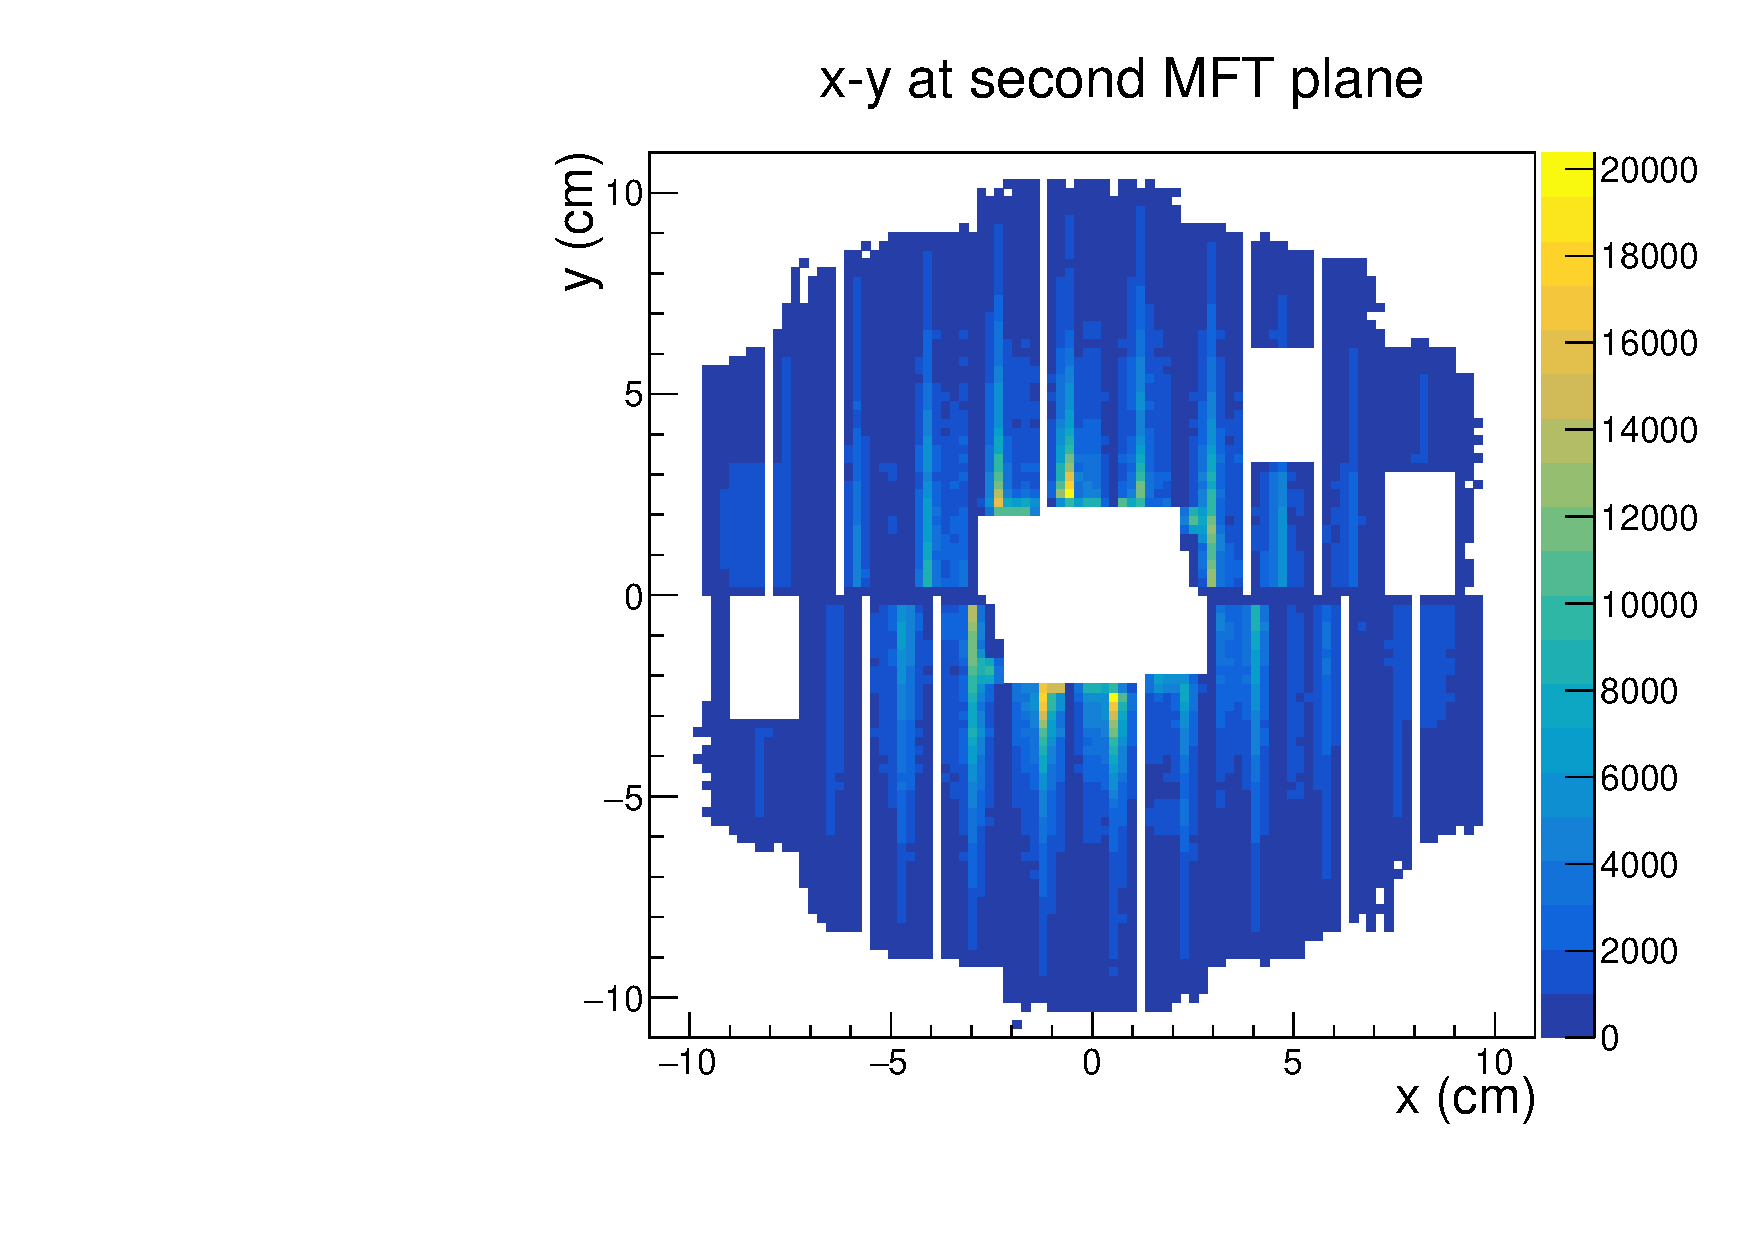
\includegraphics[width=\linewidth]{Plots/pass3_MFT/x_y_2_pass3.pdf}
        \caption{}
        \label{}
    \end{subfigure}
    \begin{subfigure}[t]{.45\linewidth}
        \centering
        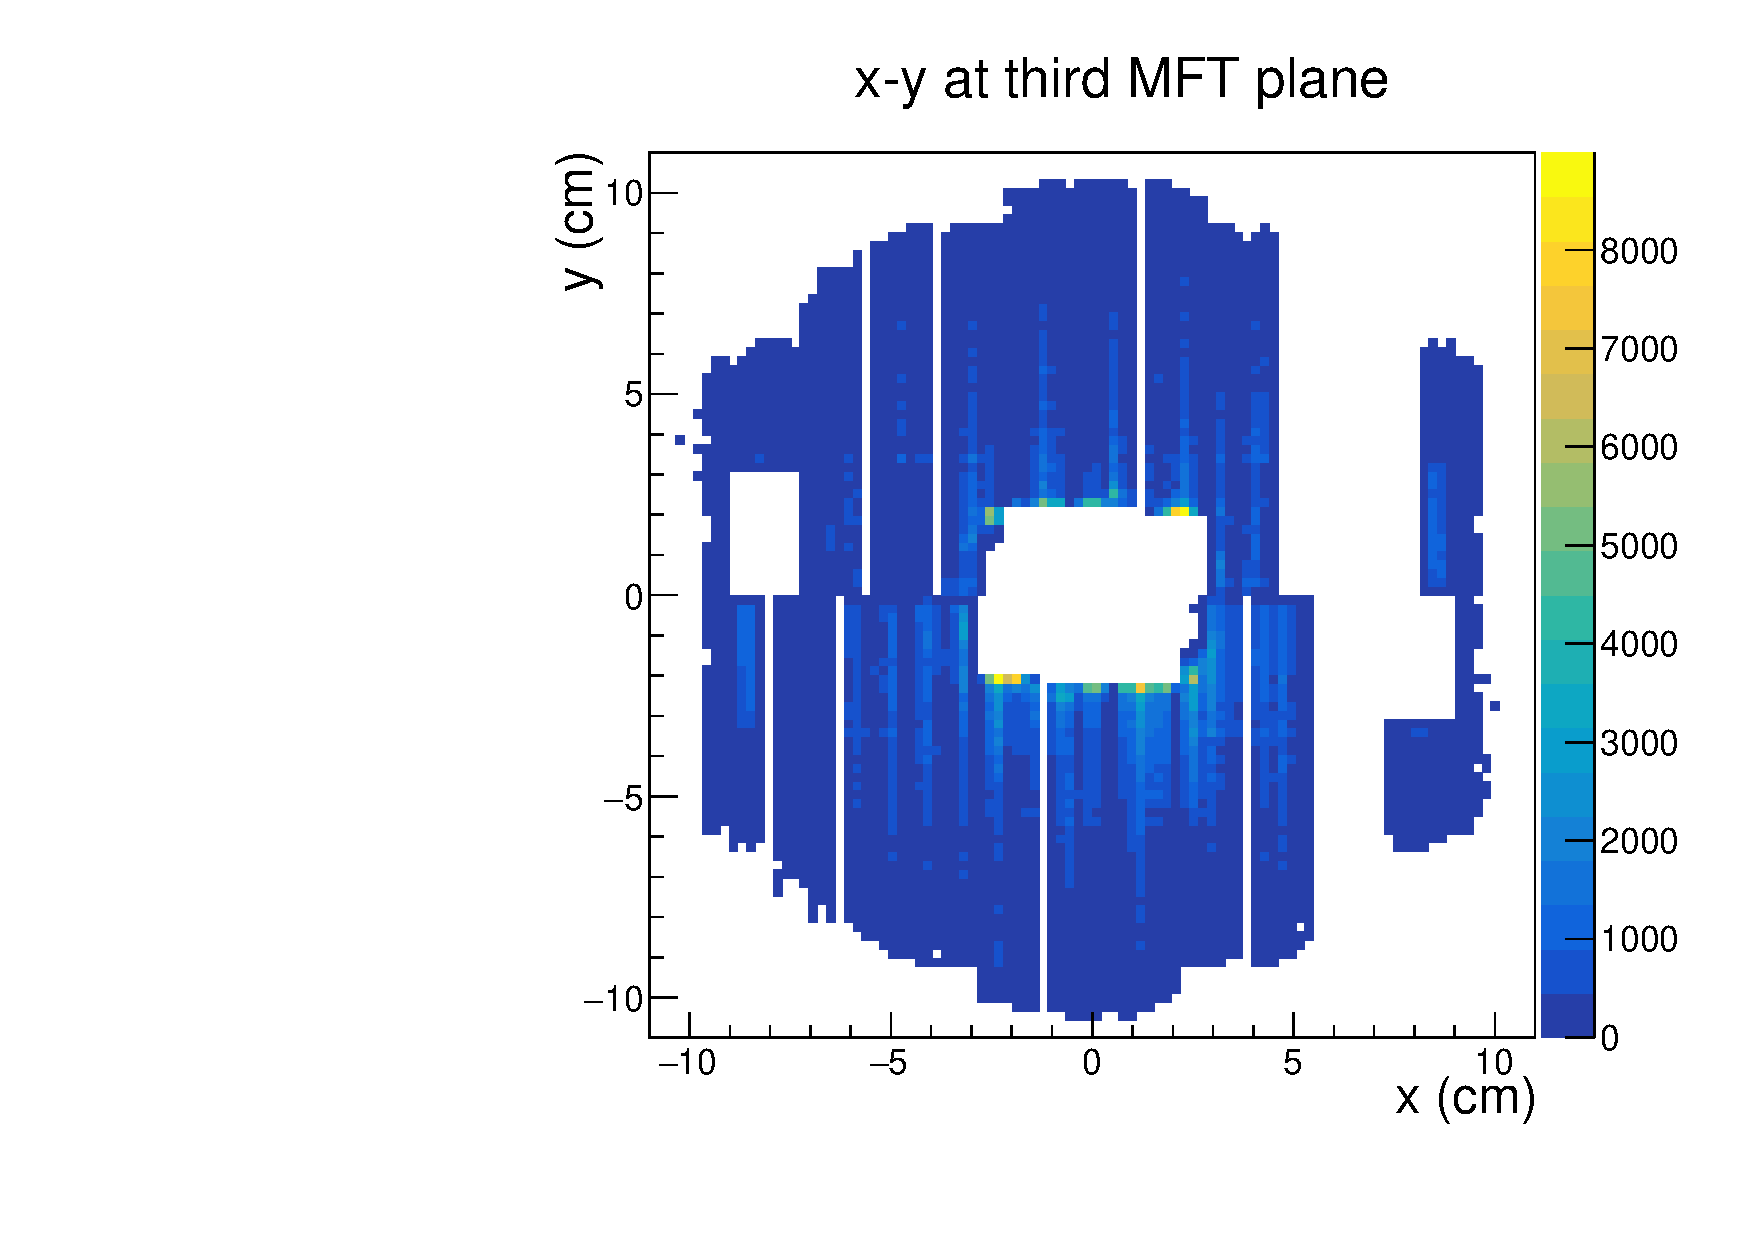
\includegraphics[width=\linewidth]{Plots/pass3_MFT/x_y_3_pass3.pdf}
        \caption{}
        \label{}
    \end{subfigure}
    \hfill
    \begin{subfigure}[t]{.45\linewidth}
        \centering
        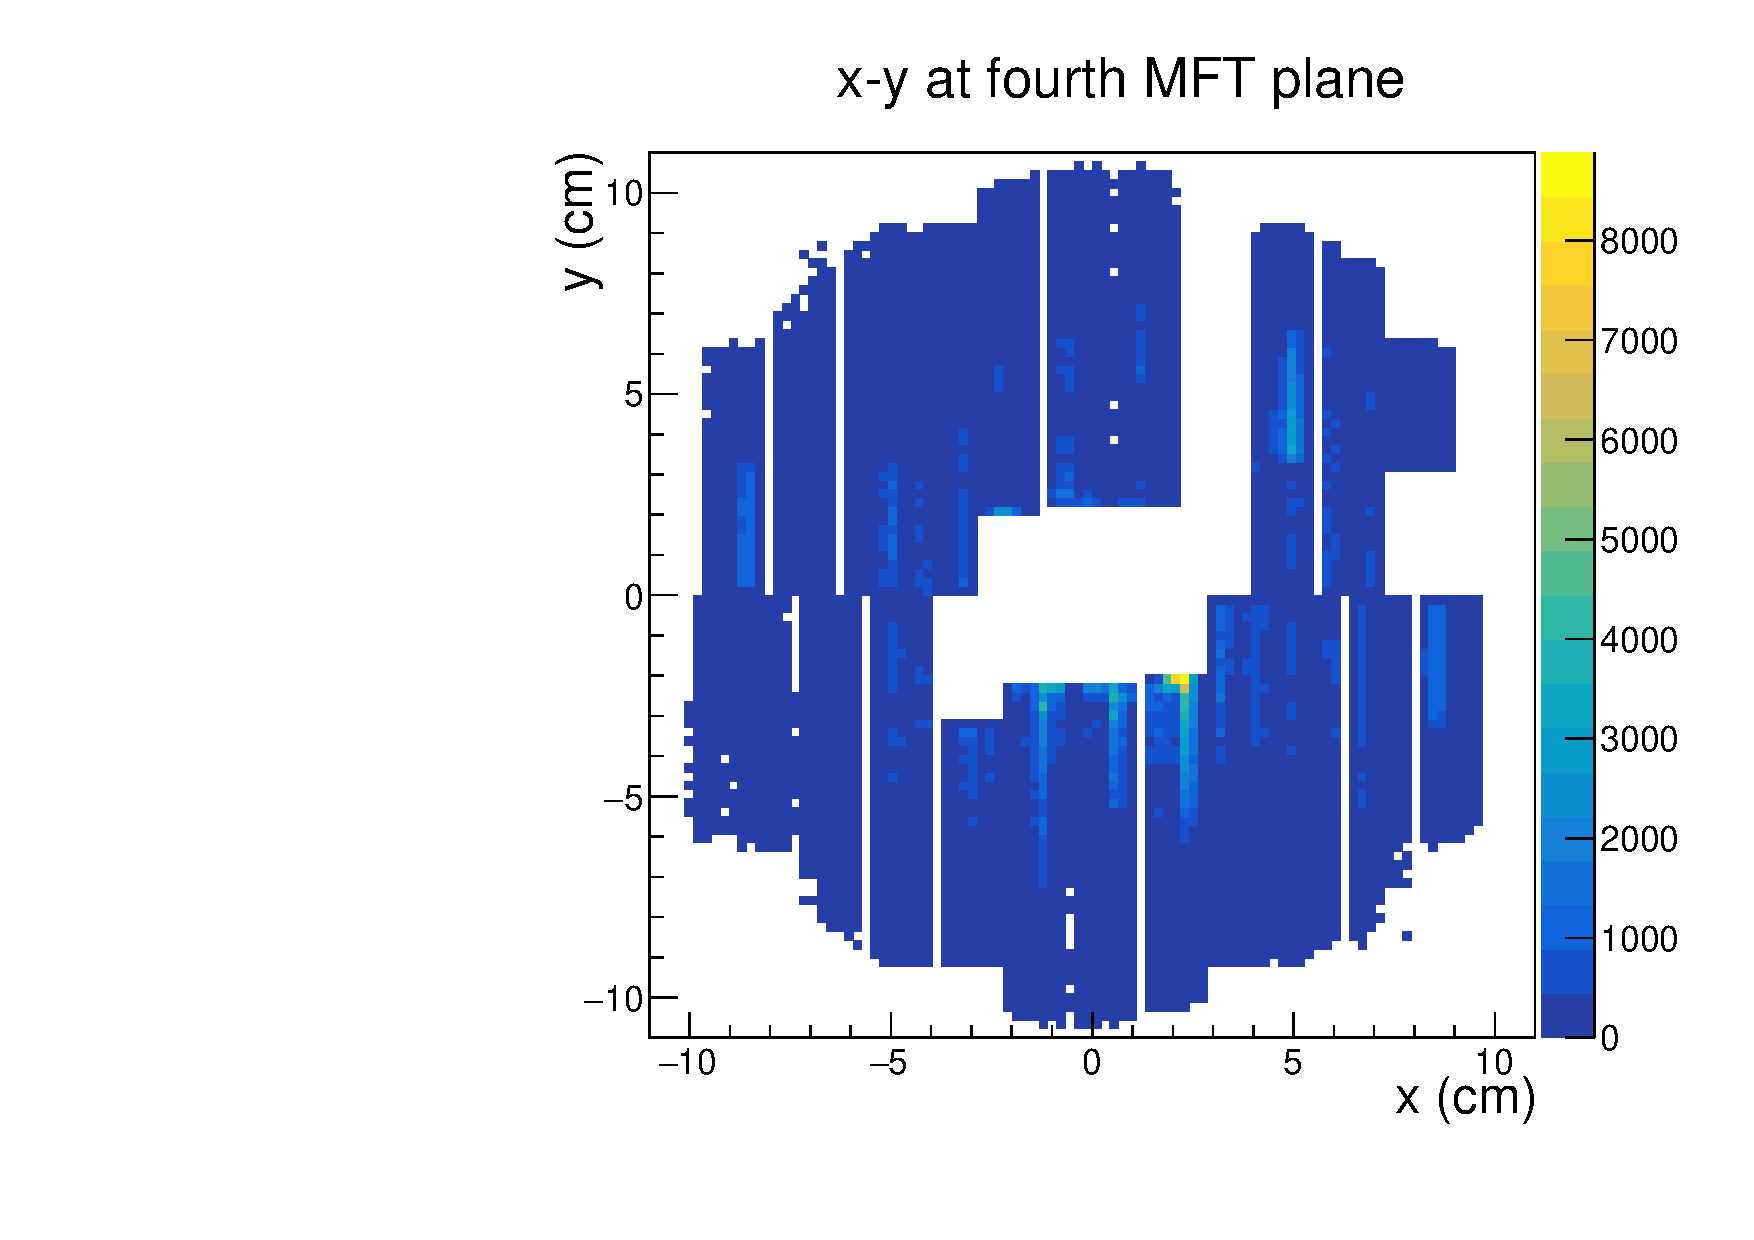
\includegraphics[width=\linewidth]{Plots/pass3_MFT/x_y_4_pass3.pdf}
        \caption{}
        \label{}
    \end{subfigure}
\caption{}
\label{fig:MFT_x_y_pass3}
\end{figure}

\subsection{Comparing pass3 to pass4}\label{sec:comapring}

\begin{figure}[h]%
    \centering
    \begin{subfigure}[t]{.49\linewidth}
        \centering
        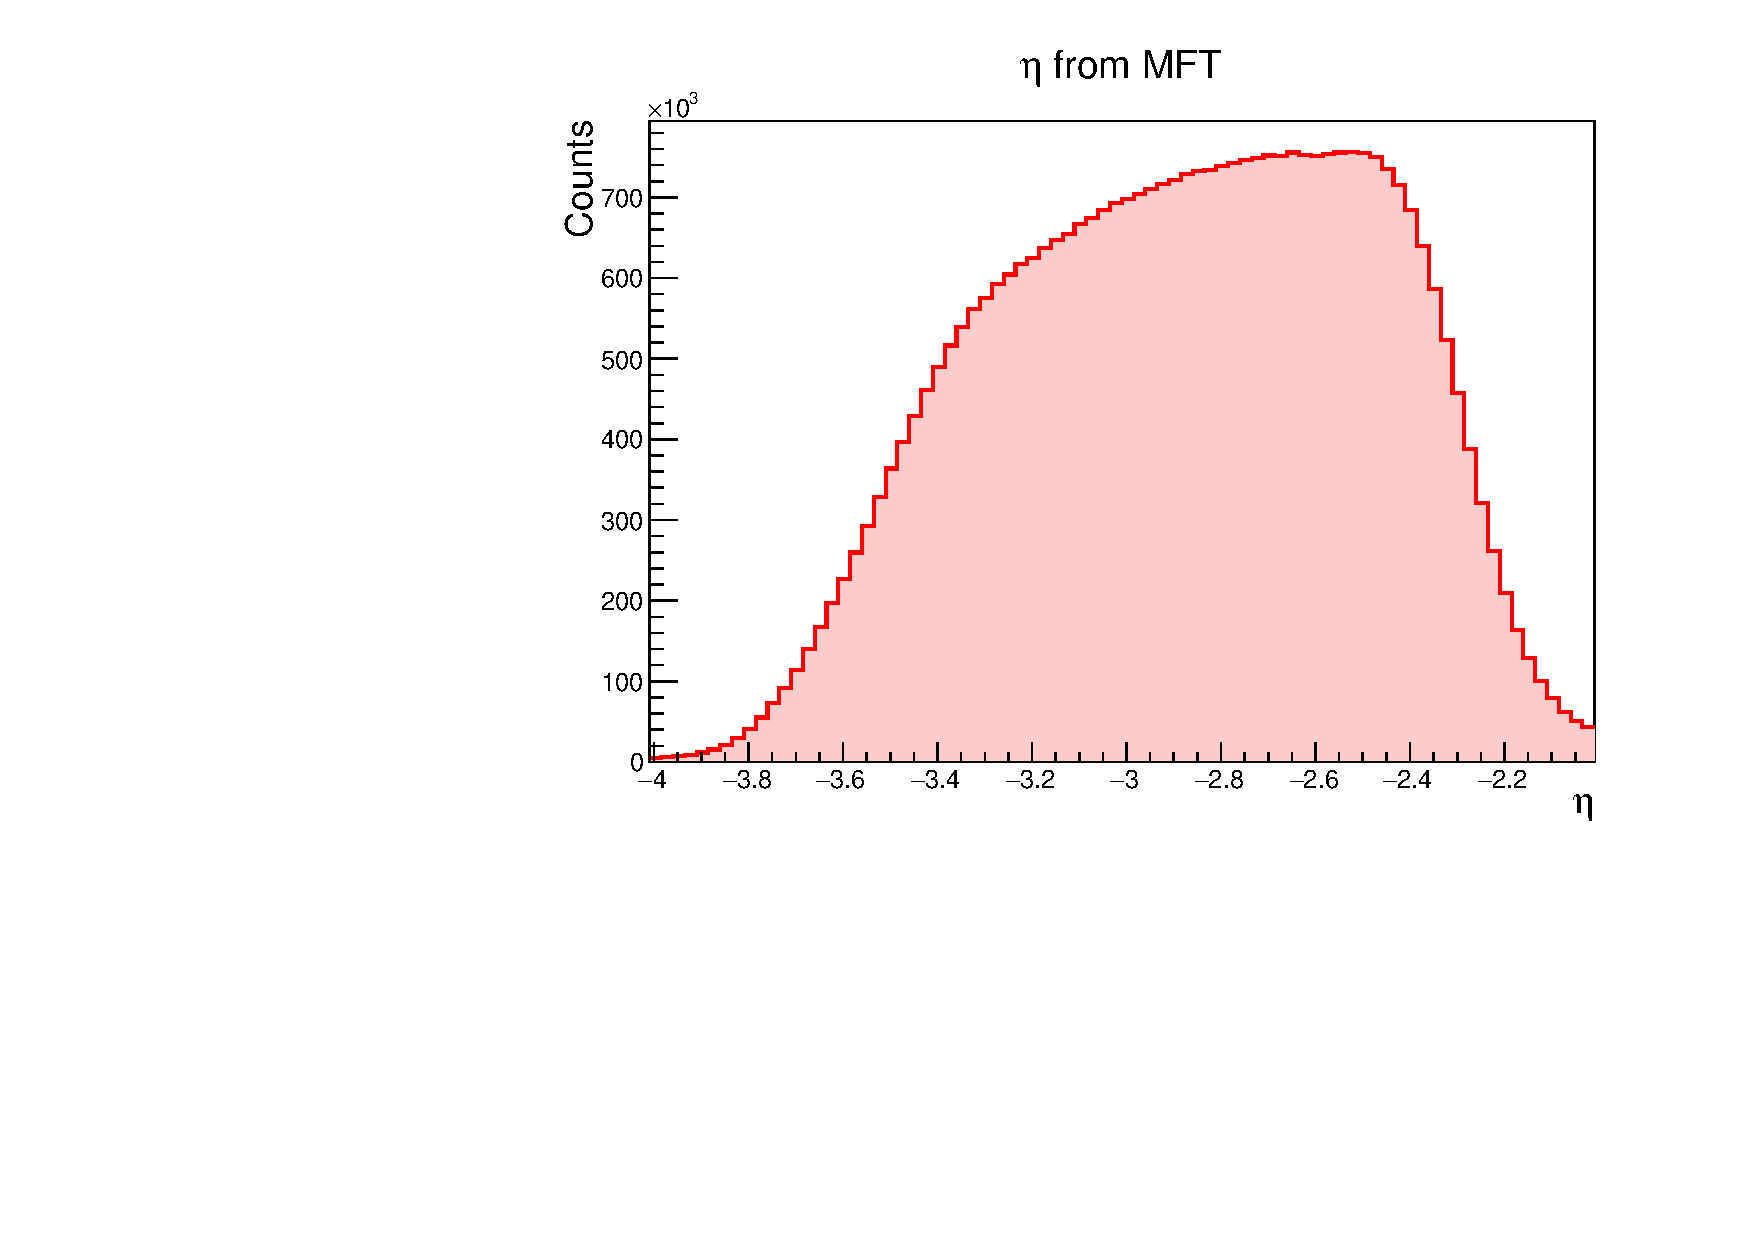
\includegraphics[width=\linewidth]{Plots/pass4_MFT/MFTeta_pass4.pdf}
        \caption{}
        \label{}
    \end{subfigure}
    \hfill
    \begin{subfigure}[t]{.49\linewidth}
        \centering
        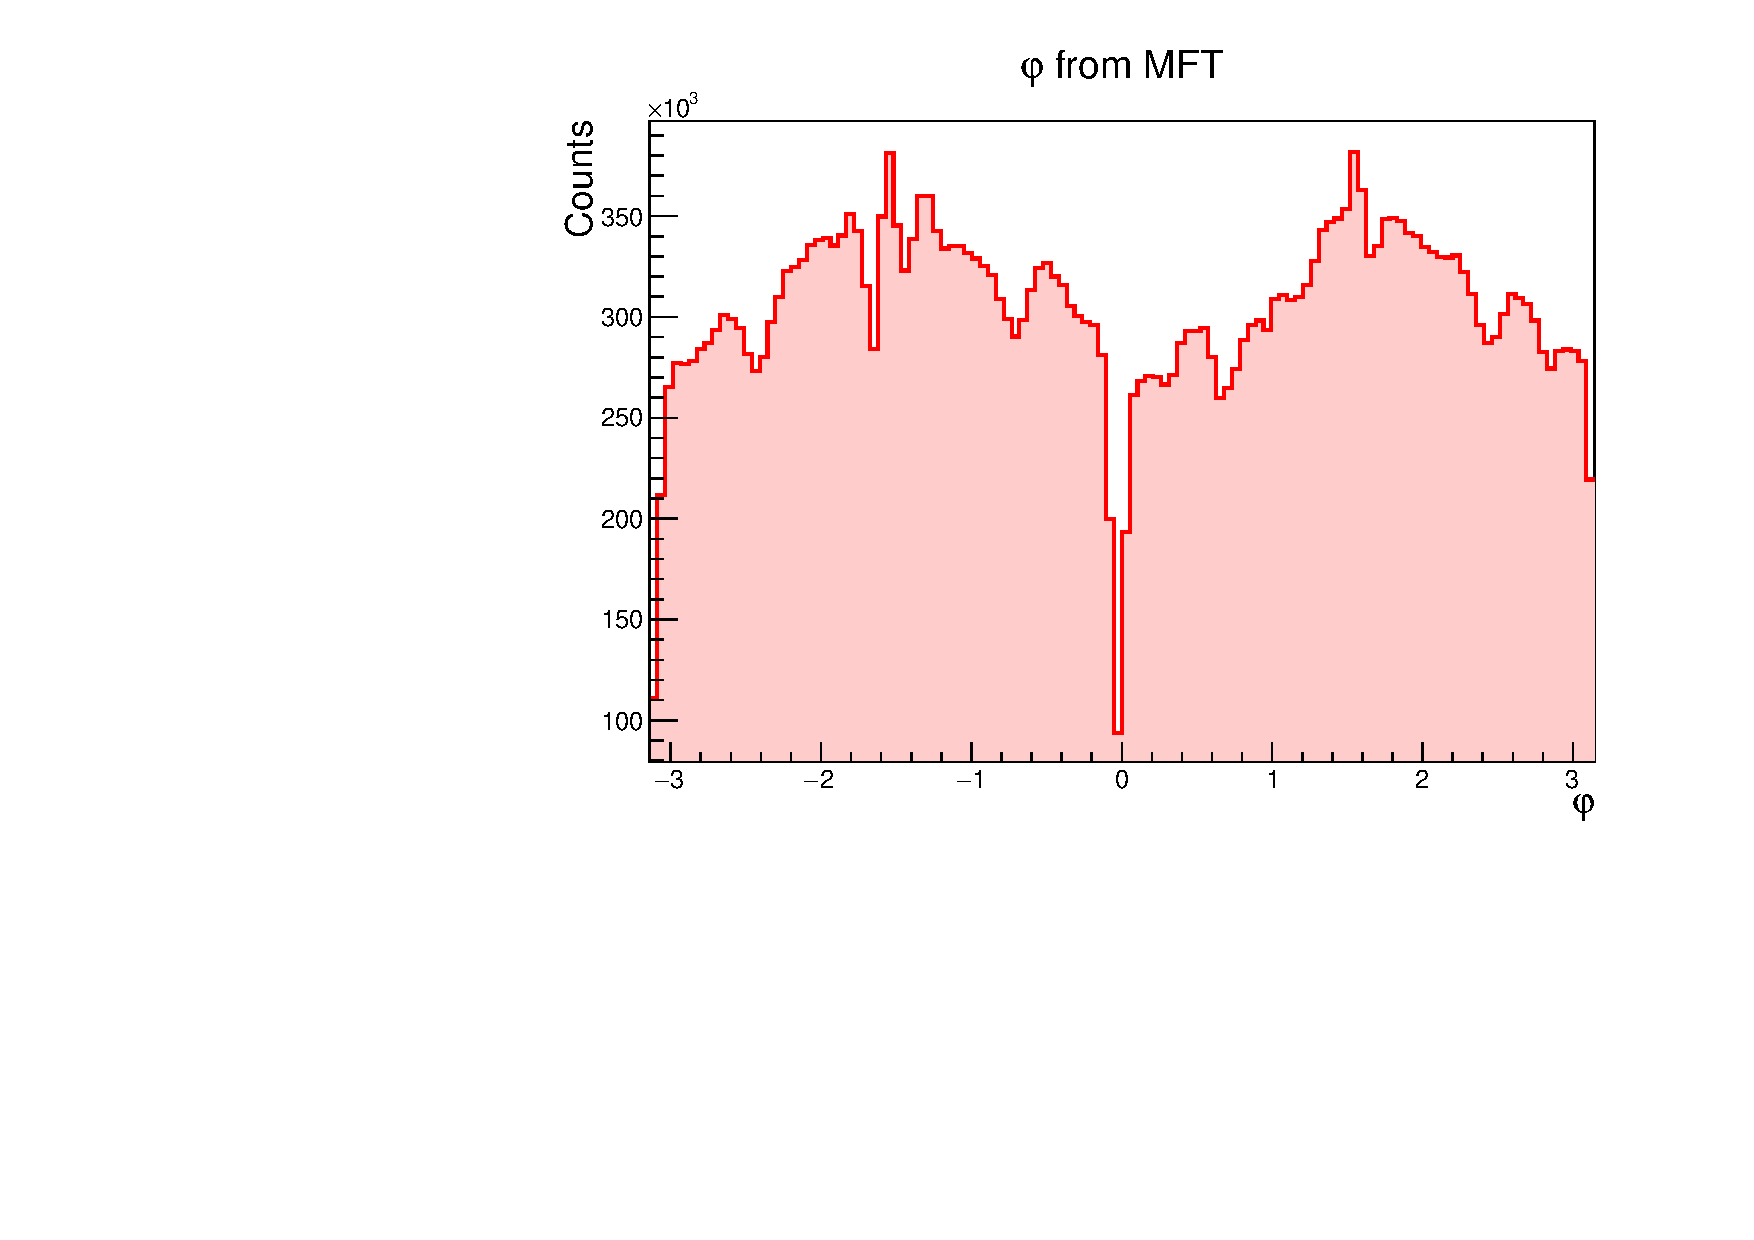
\includegraphics[width=\linewidth]{Plots/pass4_MFT/phi_pass4.pdf}
        \caption{}
        \label{}
    \end{subfigure}
    \begin{subfigure}[t]{.49\linewidth}
        \centering
        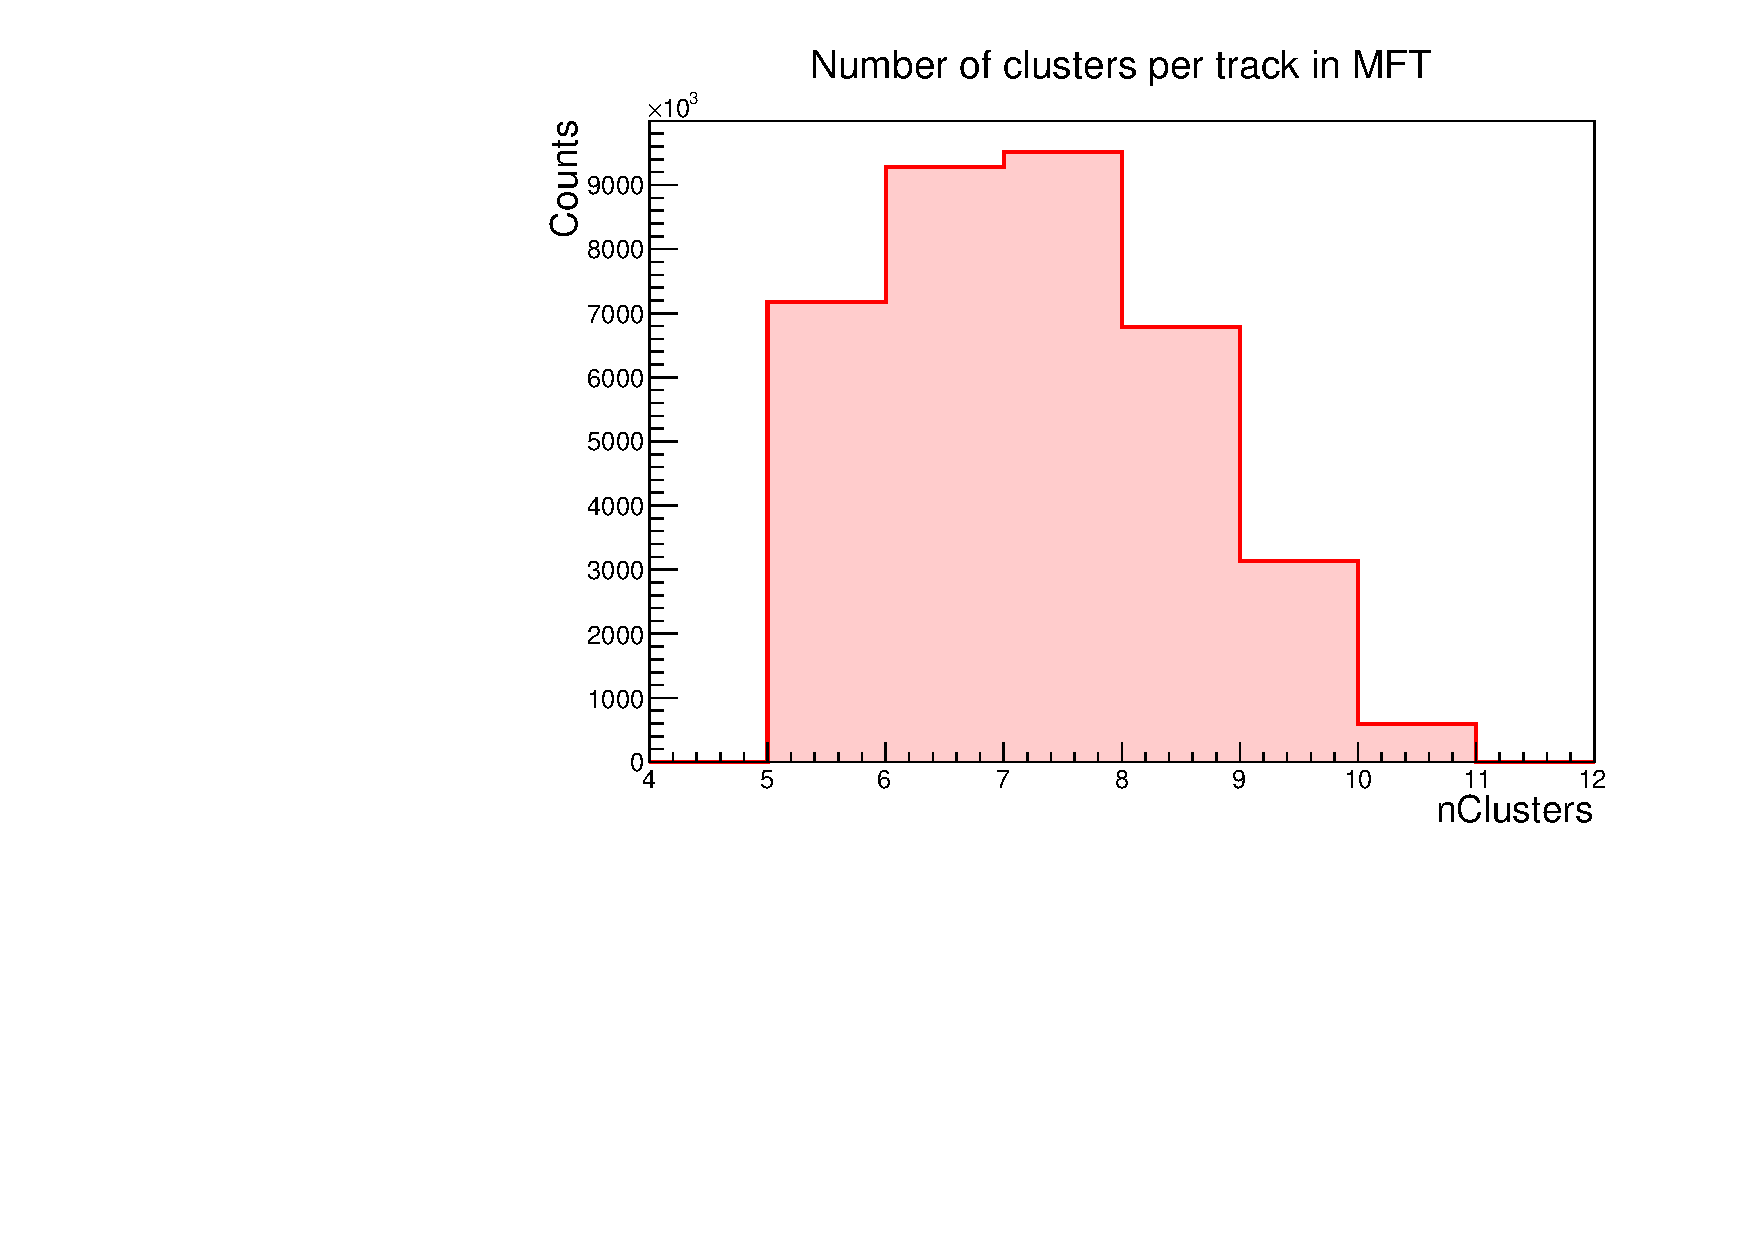
\includegraphics[width=\linewidth]{Plots/pass4_MFT/nClusters_pass4.pdf}
        \caption{}
        \label{}
    \end{subfigure}
    \hfill
    \begin{subfigure}[t]{.49\linewidth}
        \centering
        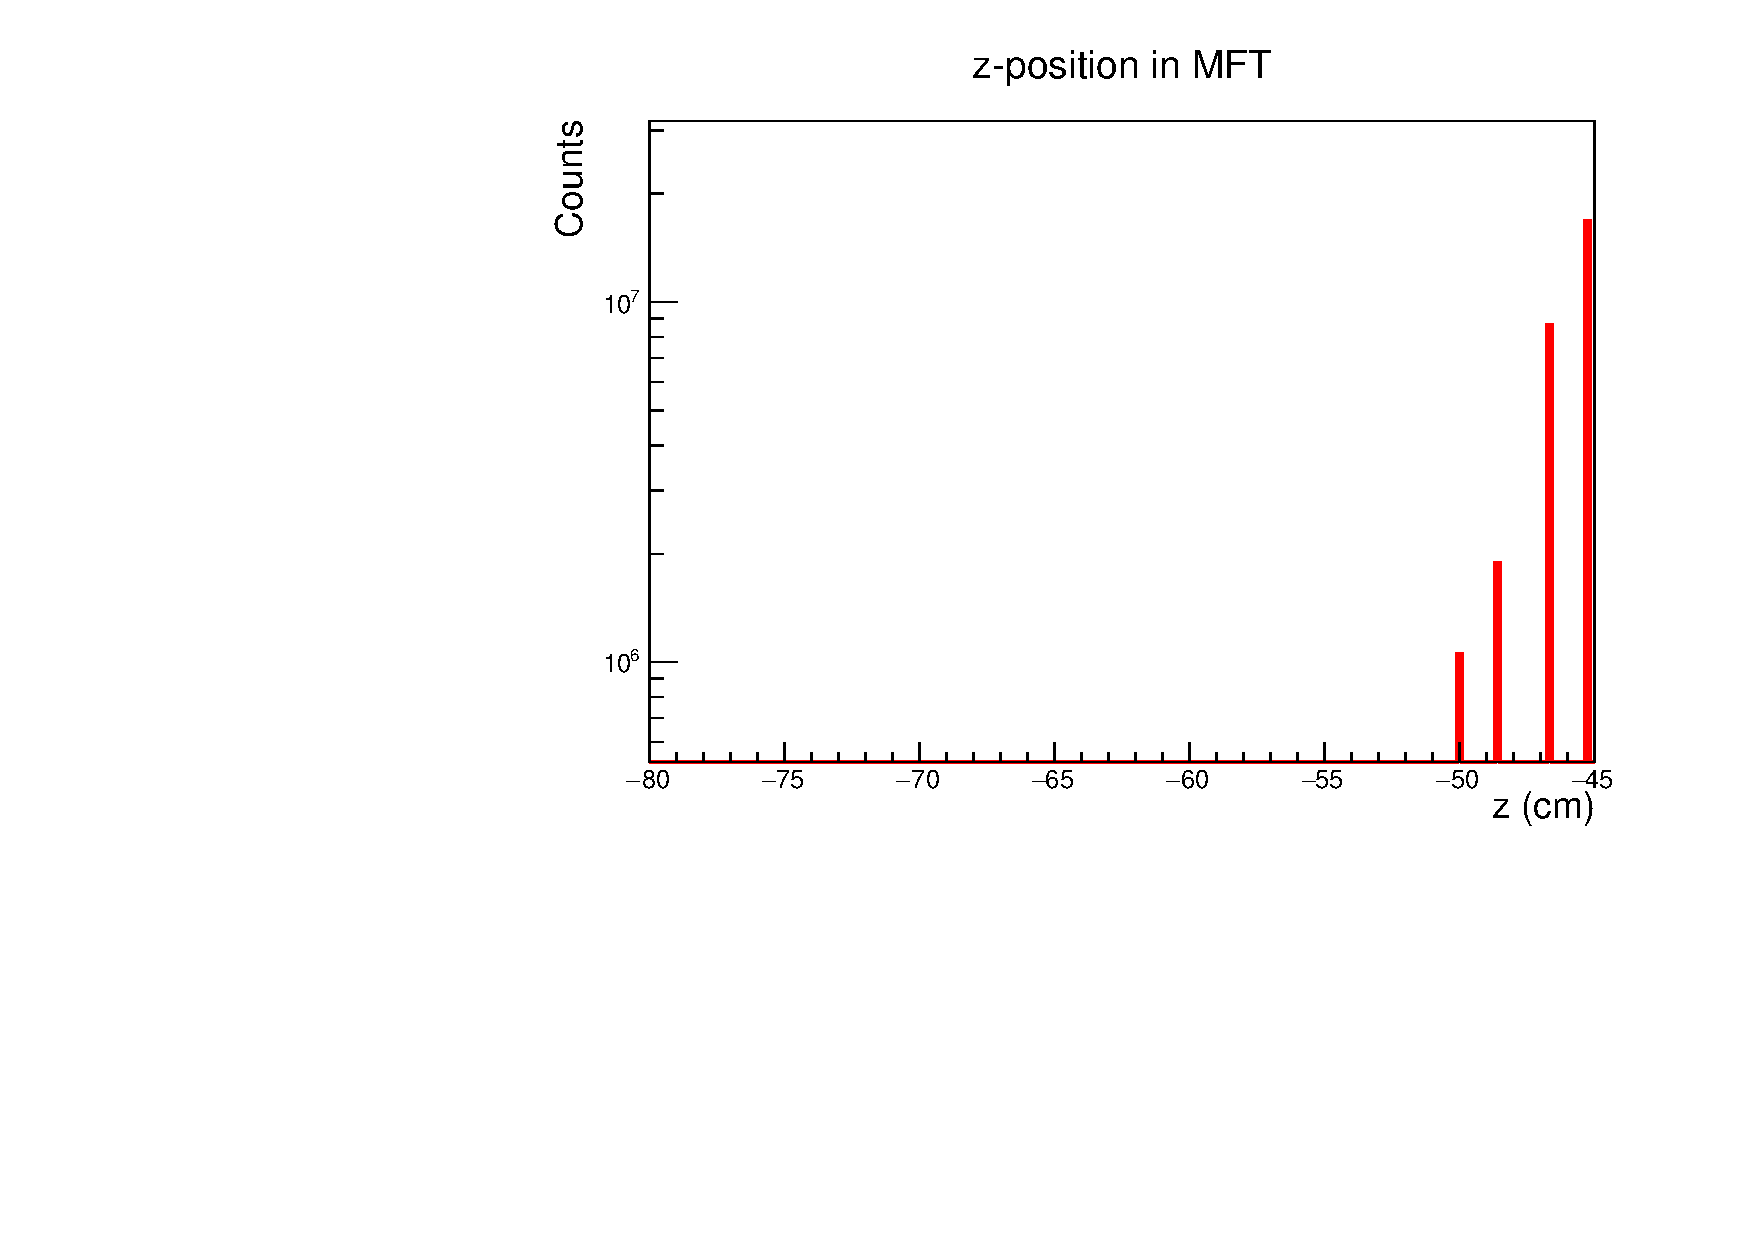
\includegraphics[width=\linewidth]{Plots/pass4_MFT/Z_MFT_pass4.pdf}
        \caption{}
        \label{}
    \end{subfigure}
\caption{}
\label{fig:MFT_1D_pass4}
\end{figure}

\begin{figure}[h]
    \begin{center}
        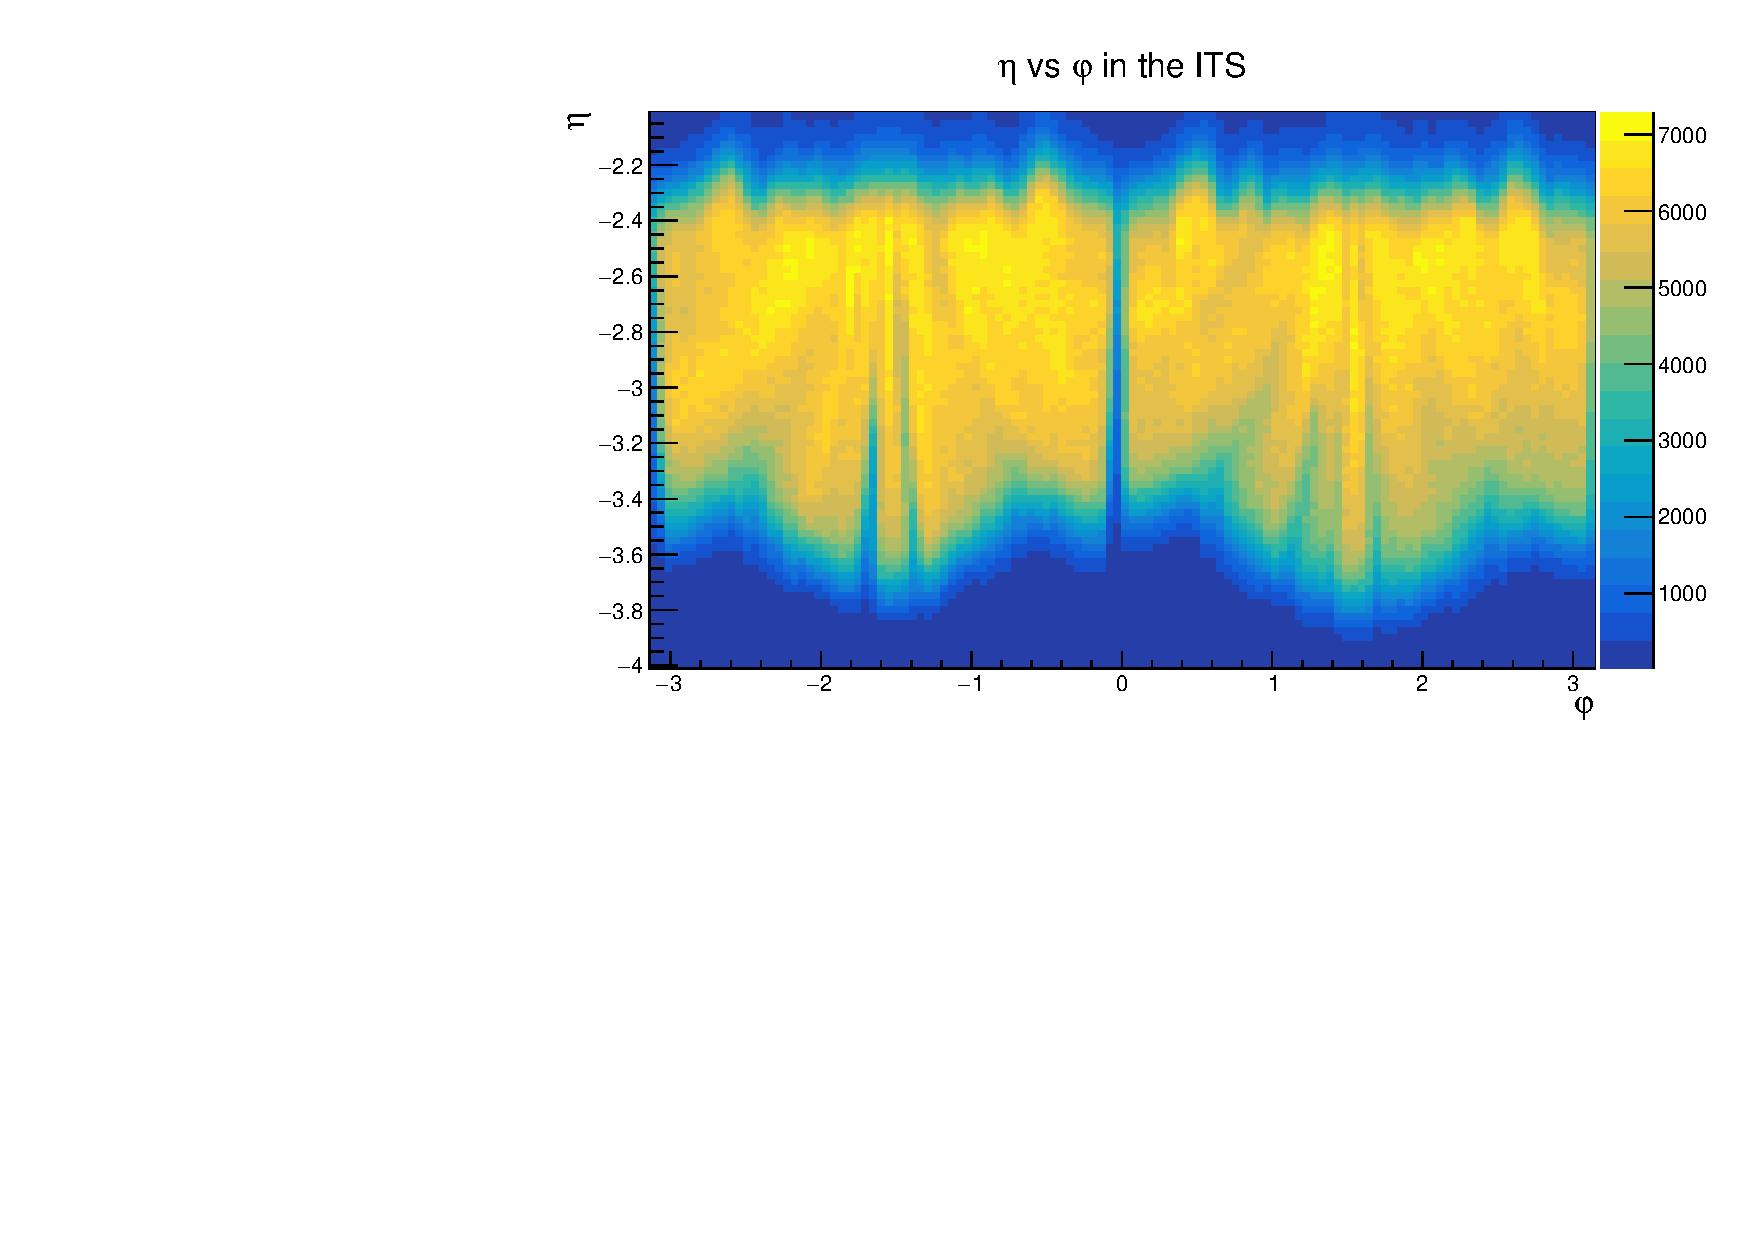
\includegraphics[width=.8\textwidth]{Plots/pass4_MFT/eta_phi_pass4.pdf}
        \caption{caption}
        \label{fig:eta_phi_pass4}
    \end{center}
\end{figure}


\begin{figure}[h]
    \begin{center}
        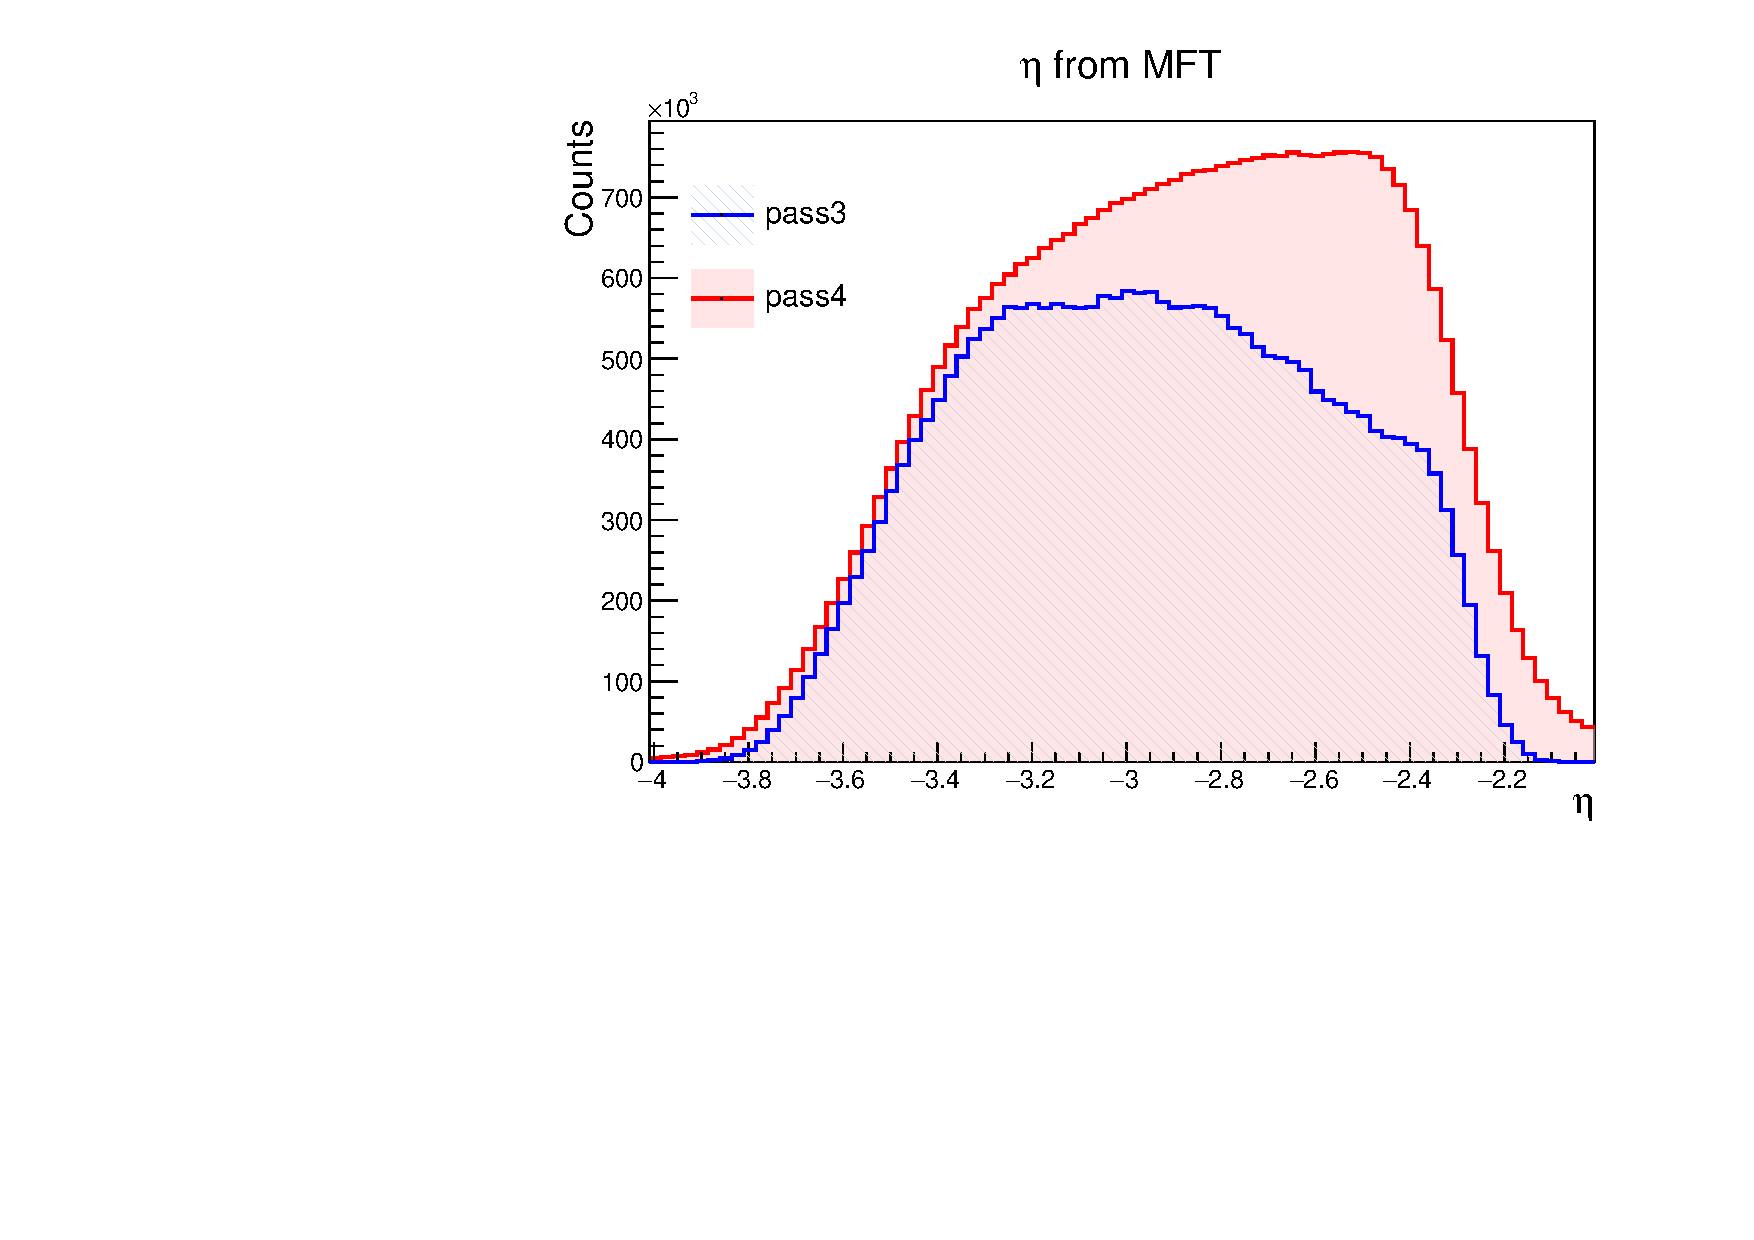
\includegraphics[width=.8\textwidth]{Plots/pass3_pass4.pdf}
        \caption{caption}
        \label{fig:pass3_pass4_eta}
    \end{center}
\end{figure}


\subsection{Initial ITS Analysis}


\subsection{Using pass4 for hasITS}